\section{Introduction to the New Model}
This chapter introduces a new ``top-down'' Continuous and Proactive Security Assessment Model (CAPSAM) framework as a response to limitations in traditional risk assessment approaches. The case study by \citet{shaikh2023information} addressed the reactive nature of the Top Management Team (TMT)'s attention in its influence on the decision to carry out an Information Security Risk Assessment (ISRA). This reveals the need for a new proactive, continuous security model that integrates information security across all layers of an organisation.

\section{Overview of the CAPSAM Framework}
    \subsection{Purpose, Goals, and Intended Outcomes}
    The CAPSAM framework is designed to \textbf{address the limitations of cybersecurity models} by emphasising a proactive and continuous approach to risk assessment. Its primary purpose is to \textbf{integrate information security considerations from the earliest stages of system development} and throughout its lifecycle.

    The main goal of CAPSAM is to minimise the likelihood and impact of cybersecurity breaches through vigilant, ongoing risk management. The model aims to \textbf{integrate information security across all layers of an organisation} and focuses on continuous improvement, ensuring a resilient security posture that adapts to the ever-changing threat landscape. By doing this, CAPSAM prioritises the protection of all stakeholders\textemdash including the customer and their data\textemdash strengthening overall organisational security and trust.

    \subsection{The Five Pillars of CAPSAM}
    The core philosophies of CAPSAM can be summarised in five pillars: \textbf{Culture, Continuous, Auditing, Response, Proactive (CCARP)}. These pillars are illustrated in Figure \ref{fig:CAPSAM_Pillars} and form the foundation of the model's approach to information security risk management.

    \begin{figure}[htbp]
        \centering
        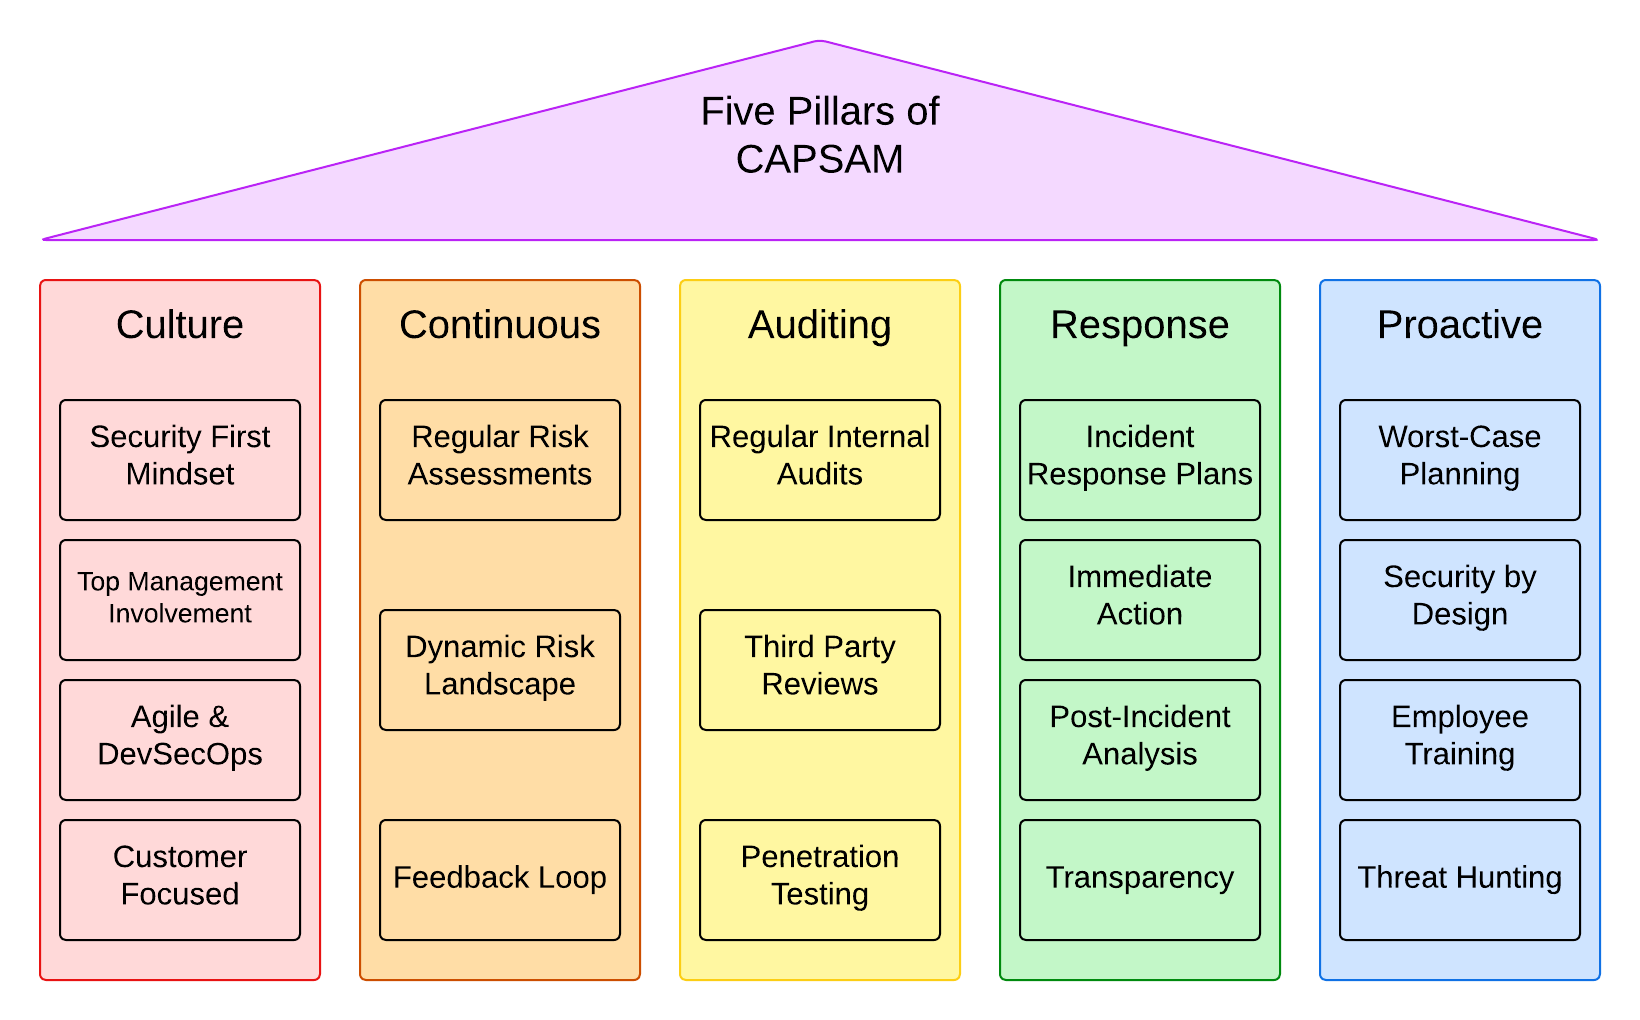
\includegraphics[width=0.8\textwidth]{figures/CAPSAM-Pillars.png}
        \caption{The Five Pillars of CAPSAM: Culture, Continuous, Auditing, Response, and Proactive (CCARP) and their components, explained in Table \ref{tab:CAPSAM_Pillars_Components} in appendices.}
        \label{fig:CAPSAM_Pillars}
    \end{figure}

    \subsection{FAMRM Cycle}
    The CAPSAM framework operates within the FAMRM cycle (New \textbf{Feature}, Information Security Risk \textbf{Assessment}, Proactive \textbf{Mitigation} Strategies, Incident \textbf{Response} Planning, and Continuous Threat \textbf{Monitoring}). This cycle ensures that each new feature or system development is subject to proactive mitigation strategies, and continuous risk assessments where feedback loops inform the next ISRA. The FAMRM cycle is illustrated in Figure \ref{fig:FAMRM_Cycle}.

    \begin{figure}[htbp]
        \centering
        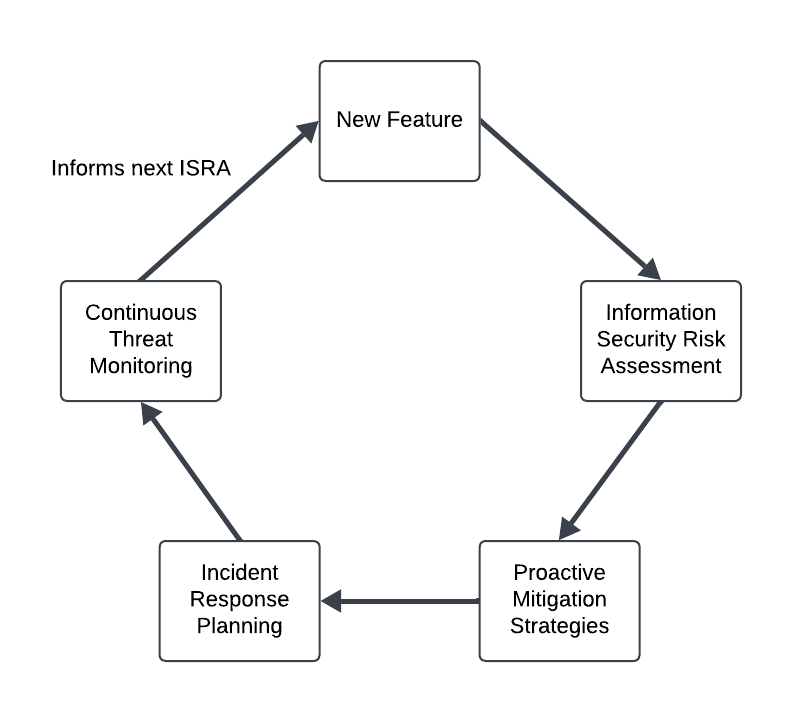
\includegraphics[width=0.6\textwidth]{figures/FAMRM-Cycle.png}
        \caption{FAMRM Cycle for Integrating Security into New Feature Development, Highlighting Continuous Risk Assessment, Proactive Mitigation, and Feedback Loops in Agile and DevSecOps Environments.}
        \label{fig:FAMRM_Cycle}
    \end{figure}

\section{Justification for a Top-Down Approach}
    \subsection{Importance of Top-Down Risk Management}
    A top-down approach is essential for embedding security as a strategic priority, ensuring executive leadership drives resource allocation and policy enforcement \citep{linkov2014risk, fazlida2015information}. While bottom-up approaches help identify technical vulnerabilities, they often lack strategic alignment, leaving broader organisational risks unaddressed \citep{linkov2014risk}. CAPSAM leverages top-down management by integrating security into governance and aligning it with business objectives, as emphasised in its `Culture' pillar.

    \subsection{Alignment with Corporate Governance}
    Aligning security with corporate governance ensures that executive management takes responsibility for protecting information assets, integrating security into organisational strategy, and fostering trust and competitive advantage \citep{fazlida2015information}. CAPSAM reflects this alignment by requiring top management involvement, as noted in its `Culture' pillar, which prioritises a security-first mindset across all levels.

    \subsection{Limitations of Bottom-Up Approaches}
    Bottom-up strategies often lack management buy-in, leading to insufficient resources and poor coordination across departments \citep{fazlida2015information, shedden2010information}. They tend to focus on technical issues while overlooking broader risks, including human error and social engineering \citep{shaikh2023information, cai2017cybersecurity}. CAPSAM addresses these limitations by embedding security into organisational culture and ensuring a proactive approach to risk management through its FAMRM cycle.

\section{Theoretical Foundations}
    \subsection{Attention-Based View (ABV)}
    The ABV theory highlights the limited attention capacity for non-routine activities, emphasising the need for strategic focus on security \citep{shaikh2023information}. CAPSAM operationalises ABV by ensuring top management prioritises cybersecurity through its `Culture' pillar. This focus increases resource allocation and fosters proactive, continuous security assessments, reducing vulnerabilities \citep{shaikh2023information}.

    \subsection{Agile Methodology and DevSecOps Principles}
    Agile and DevSecOps principles align with CAPSAM's `Continuous' pillar by enabling rapid adaptation to evolving threats and integrating security into development lifecycles \citep{ibm2021devsecops, dingsoyr2012agile}. CAPSAM's iterative risk assessments and security controls, supported by Agile's adaptability, reflect its commitment to proactive and continuous improvement.

    \subsection{ISO 31000: Risk Management Standard}
    ISO 31000 informs CAPSAM's risk management practices by advocating iterative risk evaluation and treatment \citep{purdy2010iso}. CAPSAM's FAMRM cycle incorporates these principles, emphasising continuous communication, monitoring, and adaptation to align risk management with organisational objectives \citep{purdy2010iso}.

    \subsection{Organisational Learning and Continuous Feedback}
    CAPSAM embodies organisational learning by integrating dynamic feedback loops into its FAMRM cycle \citep{murray2003continuous}. This approach enhances resilience by using insights from audits, risk assessments, and incident responses to refine security measures continually.

    \subsection{Customer-Focused Approach and Trust Theory}
    CAPSAM prioritises consumer data protection, embedding security into every development stage to build trust and align with corporate social responsibility \citep{moir2001csr, parmar2010stakeholder}. Its focus on transparency during security incidents enhances stakeholder trust, treating trust as relational capital \citep{castelfranchi2010trust}. This aligns with CAPSAM's `Culture' and `Proactive' pillars, fostering organisational credibility and resilience.

\section{Critical Analysis and Justification}
    \subsection{Strengths of CAPSAM}
    Critically analyse the strengths of the CAPSAM model, such as its proactive nature, emphasis on stakeholder engagement, and its continuous improvement cycle. Use sources to support your claims on the benefits of proactive risk management.

    \subsection{Limitations of CAPSAM}
    Acknowledge the limitations and challenges of implementing CAPSAM. Discuss aspects such as the need for continuous updates to risk assessments, the resources required for ongoing monitoring, and the potential for over-reliance on specific teams or individuals.

    \subsection{Comparison with Case Study Approach}
    Compare CAPSAM with the reactive approach in the case study. Highlight how CAPSAM's proactive, top-down, and continuous nature addresses the gaps and limitations of the case study approach.

    \subsection{Challenges in Implementing CAPSAM}
    Discuss potential challenges in implementing CAPSAM, such as obtaining management support, ensuring consistent communication across departments, and managing the resources needed for continuous monitoring.

\section{Implementation of CAPSAM}
    \subsection{Phase 1: Planning and Preparation}
    Outline the first phase of implementing CAPSAM, which involves identifying key stakeholders, defining roles and responsibilities, and establishing communication channels. Discuss the importance of aligning the security risk management policy with the organisation's overall strategy.

    \subsection{Phase 2: Implementation}
    Describe the process of conducting risk assessments, identifying vulnerabilities, prioritizing risks, and developing mitigation strategies. Explain the importance of integrating risk management activities with the software development lifecycle.

    \subsection{Phase 3: Review and Improvement}
    Detail the review phase, which involves regular assessments of the CAPSAM framework, adapting the model based on insights and business changes, and fostering a culture of continuous security improvement.

\section{Conclusion}
Summarize the key points discussed in the chapter, reinforcing the value of the CAPSAM framework in overcoming the limitations of traditional risk assessment models. Emphasize the importance of a proactive, continuous approach to information security and its alignment with business practices and strategic goals.